% -*- fill-column: 85; -*-
%!TEX root = ../dissertation.tex
\section{Background}
\label{s:background}


Cloud providers currently support compute accelerators using PCIe pass-through, which dedicates the device exclusively to a single guest.
Despite evidence of accelerator under-utilization~\cite{underutilizingcloud,simultaneous_multikernel,improving_gpu,gpl,fiddle}, and abundant
research~\cite{simultaneous_multikernel,improving_gpu,gpl,fiddle,zhang2018g,yeh2017pagoda}, no practical alternative yet exists.
This section provides background to explain this trend and motivates \Model's design.

\subsection{Virtualization Properties}
\label{s:properties}

Virtualization is a huge area---see~\cite{bugnion_neih_tsafrir} for comprehensive treatment.
We focus on properties critical for accelerator virtualization: \emph{interposition}, \emph{compatibility}, and \emph{isolation}.

\paragraphbe{Interposition.}
Virtualization decouples a logical resource from a physical one
through an indirection layer, intercepting guest interactions with
a virtual resource and providing the requested functionality using
a combination of software and the underlying physical resource.
Thus, virtualization works by \emph{interposing}
an interface, and changing or adding to its behavior.
Interposition is fundamental to virtualization and provides well-known benefits~\cite{waldspurger-iovirt}.
The choice of interface and the mechanism for interposing it
profoundly impacts the resulting system's practicality.
\emph{Inefficient} interposition of an interface (e.g. trapping frequent MMIO access) undermines
performance~\cite{suzuki2014gpuvm,yufull}; \emph{incomplete} interposition
compromises the hypervisor's ability to enforce isolation.
%If an interposed interface does not completely encapsulate the underlying resource,
%isolation may be lost.~\cjr{maybe ditch that last one.}

\paragraphbe{Compatibility} captures multiple related dimensions, including
robustness to evolution of interposed interfaces and adjacent stack layers,
and applicability across multiple platforms or related devices.
For example, full virtualization of a accelerators's hardware interface (\S\ref{s:bg_tech})
has \emph{poor} compatibility in that it works only with that device.
However, it has \emph{good} compatibility with guest software,
% (Table~\ref{tab:virt-comp}),
which will work without modification.
%, assuming the operating system has
%appropriate drivers for the device.
Current accelerator virtualization techniques
reflect a compromise between these two forms of compatibility.
%\Model gives up
%guest software compatibility, but compensates for that loss with automation (\S\ref{s:compiler}) to quickly
%adapt to software and hardware evolution (\S\ref{s:design}).


\paragraphbe{Isolation.} Cross-VM isolation is a critical requirement for
multi-tenancy:
when a resource is multiplexed among mutually distrustful tenants,
tenants must not be able to see/alter each other's data (\emph{data isolation}),
or adversely affect each other's performance (\emph{performance isolation}).
A poor choice of interposition mechanism and/or interface limits the system's ability to provide these guarantees: e.g., API remoting~\cite{bitfusion, rCUDA, mps}
%\amp{``often''?}
%\cjr{always}
%forwards interposed API calls from VMs to a shared remote server,
can have poor isolation (\S\ref{s:bg_api_remoting}) because the hypervisor is bypassed.
%Using separate servers for each protection provides isolation.

\begin{figure}[!t]
	\centering
	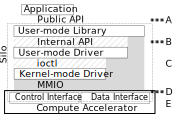
\includegraphics[width=.78\linewidth]{ava/images/silo.pdf}
	\caption{An accelerator silo.
		The public API and the interfaces with striped backgrounds are interposition candidates.
		All interfaces with backgrounds are proprietary and subject to change.
        %\cjr{Ref \S\ref{s:bg_tech} here?}\amp{Arrows removed to match more traditional idea of stack diagram and simplify drawing. Someone please second this choice.}
        %\cjr{seconded. Thanks!}
        }
	\label{fig:silo}
\end{figure}

\subsection{Accelerator Silos}
\label{s:silo}

% Accelerator vendors develop commodity software stacks
% using a common set of techniques.
Accelerator stacks
compose layered components that include a user-mode library to support an
API framework and a driver to manage the device.
Vendors are incentived to use proprietary interfaces and protocols between layers to preserve forward compatibility,
and to use kernel-bypass communication techniques to eliminate OS overheads.
However, interposing opaque, frequently-changing interfaces communicating with memory
mapped command rings is \emph{impractical} because it requires inefficient techniques and
yields solutions that sacrifice compatibility.
Consequently, accelerator stacks are effectively \emph{silos}
(Figure~\ref{fig:silo}), whose intermediate layers
\emph{cannot be practically separated} to virtualize the device.

\paragraphbe{Current support.} Most current hardware
accelerators feature some hardware support for virtualization: primarily for process-level
address-space separation, and in a small handful of cases, SR-IOV (\S\ref{s:bg_tech}).
A central premise of this paper is that hardware support for process-level isolation \emph{could}
suffice to support hypervisor-level virtualization as well, but the siloed structure of current accelerator stacks prevents it.

\begin{comment}
\begin{figure}[!t]
	\centering
  \vspace{-0.5em}
	\includegraphics[width=.75\linewidth]{ava/data/rate_limit/qat_unfairness.pdf}
    \vspace{-.2cm}
	\caption{Throughput achieved by three instances of QATzip (running in VMs with SR-IOV pass-through) with different block sizes, running separately (\textbf{\texttt{Uncontended}}) and concurrently (\textbf{\texttt{Contended}}). Slowdown during concurrent execution is dependent on block size, i.e., the QAT HW scheduler cannot guarantee fairness.}
	\label{fig:qat-unfairness}
\end{figure}
\end{comment}

\subsection{Existing Accelerator Virtualization Techniques}
\label{s:bg_tech}


%% !TeX root = ../main.tex
\begingroup % Prevent leakage of length settings and defs into other files.

\def\chk{\checkmark}

\begin{table}[]
\resizebox{\columnwidth}{!}{%
\begin{tabular}{c|c|c|c|}
\cline{2-4}
                                      & isolated & interposition & compatibility \\ \hline
\multicolumn{1}{|l|}{PCIe PT}         &          &               &               \\ \hline
\multicolumn{1}{|l|}{FV}              & \chk     & \chk          &               \\ \hline
\multicolumn{1}{|l|}{MPT}             & \chk     &               &               \\ \hline
\multicolumn{1}{|l|}{PV}              & \chk     & \chk          &               \\ \hline
\multicolumn{1}{|l|}{SR-IOV}          & \chk     &               & \chk          \\ \hline
\multicolumn{1}{|l|}{API-Remote}      &          &               &               \\ \hline
\multicolumn{1}{|l|}{HIRA}            & \chk     & \chk          &               \\ \hline
\multicolumn{1}{|l|}{Automation+HIRA} & \chk     & \chk          & \chk          \\ \hline
\end{tabular}
}
\caption{
	Properties of virtualization techniques.
}
\label{tab:tech_compare}
\end{table}
%\hyu{Table~\ref{tab:tech_compare}}

%%% For accelerators, conventional virtualization techniques can be broadly classified according
%%% to which interface(s) they interpose (see Figure~\ref{fig:silo}) and which techniques are used to synthesize the
%%% virtual functionality.

\paragraphbe{PCIe pass-through}
is the current \emph{de facto} standard technique for exposing an accelerator to guest VMs.
It works by dedicating the hardware interface directly to the guest. Consequently,
it does not interpose \emph{any} interface. All benefits of virtualization are lost,
but native performance is preserved.

\paragraphbe{Full virtualization (FV)}~\cite{kvmgt,suzuki2014gpuvm,gVirt} interposes the hardware interface
(D in Figure~\ref{fig:silo}). For accelerators, this interface is memory mapped I/O (MMIO),
necessitating trap-based interposition (e.g. using memory protection or deprivileging), which
devastates performance (e.g., 100$\times$ or more~\cite{suzuki2014gpuvm, yufull}).
Accelerator hardware interfaces are proprietary and device-specific, so FV has poor compatibility,
even across different devices of the same type (e.g. AMD vs NVIDIA GPUs).
%Further full virtualization solutions rely on reverse-engineering of proprietary control interfaces, rendering them extremely tedious to build, maintain and evolve.

\paragraphbe{Mediated pass-through (MPT)} is a hybrid of pass-through and full virtualization.
MPT~\cite{gVirt,mdev-mvme,vpio}
uses pass-through for data plane operations, and provides a privileged
control plane interface for sensitive operations (D in Figure~\ref{fig:silo}).
MPT can preserve some of the raw speedup of
acceleration and allows guests to use native drivers and libraries.
However, limited interposition limits a hypervisor's ability to effectively manage resource sharing.
More importantly, hardware support is required and,
to our knowledge, Intel integrated GPUs are the only accelerators to support MPT~\cite{gVirt}.

\paragraphbe{Para-virtualization (PV)}
\emph{creates} an efficiently interposable interface in software and adjusts adjacent stack
layers to use it, rather than interposing an existing interface in the stack.
This necessitates a custom driver and library in every
supported guest OS for the virtual device.
The technique is powerful because enables encapsulation of diverse hardware
behind a single interposable interface.
However, compatibility is compromised: guest library and OS modifications are required,
and the para-virtual device interface must be maintained as interfaces evolve.
For example, VMware's SVGA II~\cite{svga} encapsulates
multiple GPU programming frameworks, but keeping up with the evolution of
those frameworks has proved untenable: SVGA remains multiple versions behind current frameworks~\cite{vmware_version,svga_guest} (e.g., DirectX~12~\cite{directx_version}).

\begin{comment}
\begin{figure}[!t]
	\centering
	\includegraphics[width=.8\linewidth]{ava/data/rate_limit/bf_unfairness.pdf}
	\caption{Unfairness in slowdown between \lstinline|needle| and \lstinline|hotspot| applications in separate VMs running GPU kernels iteratively
    with BitFusion FlexDirect and \model.
    % When running alone, \lstinline|hotspot| has throughput of 126.3~ms/kernel.
    Fairness is calculated by $\left|s_1-s_2\right| \mathbin{/} (s_1+s_2),$
    where $s_i$ is the slowdown of application $i$ when running concurrently.}
	\label{fig:bitfusion_unfairness}
\end{figure}
\end{comment}

\paragraphbe{SR-IOV.}
Accelerators with PCIe SR-IOV~\cite{sriov} present multiple virtual devices (VFs) to system software.
%and the \emph{hardware} shares physical resources among them.
SR-IOV provides an interface and protocol for managing VFs, but the device vendor must \emph{implement} any cross-VF sharing support (E in Figure~\ref{fig:silo}) \emph{in silicon}.
The technique can provide strong virtualization guarantees~\cite{dong2012high,dong2008sr}, but hardware-level resource management
is inflexible and unevolvable: current implementations are trivially vulnerable to fragmentation and unfairness pathologies that cannot be changed.
Moreover, evidence is scant that broad SR-IOV support will emerge for accelerators:
only two current GPUs support it~\cite{amdfirepro,nvidiagrid}, none of the TPUs we evaluate support it;
and SR-IOV \emph{interface} IP blocks from FPGA vendors (used by~\cite{vu2014enabling,zazo2015pcie,vfpgamanager,huang2009fpgavirt}) do not implement resource management.
We do not expect this to change any time soon:
SR-IOV requires significant engineering effort vendors are not incentivized to invest.

\begin{figure*}[!!thp!]
	\centering
    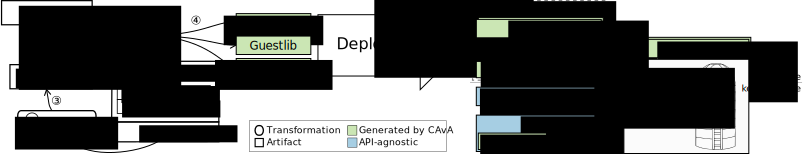
\includegraphics[width=\textwidth]{ava/images/overview.pdf}
    \caption{Overview of \model.
    %\hyu{The green and blue look the same when printed out.}
    %\amp{I don't see this problem. I increased contrast earlier today. check again?}
    %\hyu{Transport device is generated as well?}
    %\amp{Chris wanted it this way. The idea is to make the point that you need a new one for every API.}
    %\hyu{Color: it's better with my home printer but still hard to tell the difference from the legend. Device: then it conflicts with the text (\S4.1). I thought only the transport driver was generated for every API, but not the transport device.}
    %\cjr{this has converged.}
      %\amp{Tweaks if there is time: Remove extremely pale background on silo box. Separate colors more in brightness.}
    }
    \label{fig:overview}
    \vspace*{-1em}
\end{figure*}

\begin{comment}
\paragraphbe{Why is SR-IOV not the solution?} Full-featured SR-IOV from all accelerators is an unrealistic demand.
% Resource management must be baked into hardware;
Hardware designers tend to favor simple resource management policy implementations, easily leading to pathologies.
To illustrate the problem, we measured the throughput achieved by three VMs using Intel QuickAssist~\cite{QAT} (with SR-IOV) to compress data (offloaded with different chunk sizes), with and without contention (shown in Figure~\ref{fig:qat-unfairness}).
Each VM was assigned a PCIe Virtual Function (VF) exposed by the same Physical Function (PF), causing the hardware to schedule requests round-robin.
% The VMs offloaded compression in differing chunks ().
When there is no contention, each application achieves a similar throughput.
% ($\sim$17~Gib/s).
However, when the 3 applications were executed concurrently, the throughput achieved was a function of offload chunk size used, \emph{yielding unfairness that cannot be fixed without changing the hardware}.
%We argue that even if all accelerators were to provide SR-IOV, similar pathologies
%due to lost interposition and inflexible hardware-policy would be inevitable.
\end{comment}

\label{s:bg_api_remoting}
\label{s:bitfusion}
\paragraphbe{API Remoting}~\cite{gVirtuS,gupta2009gvim,VCL,duato2009efficient,li2011gpu,GridCuda,cu2rcu,xiao2012transparent,gupta2011pegasus,vcorfu}
interposes the top of the stack, between application and framework library (A in Figure~\ref{fig:silo}).
Similar to system call interposition~\cite{paradice, nooks, rio, vrio},
API calls are intercepted and forwarded to a user-level API framework~\cite{vCUDA} in an appliance VM~\cite{vmCUDA}, or remote server~\cite{rCUDA,kim2012snucl}.
Limited interposition frequency, batching opportunities~\cite{rCUDA} and high-speed networks~\cite{deplyrcuda, bitfusion} reduce overheads,
making it appealing to industry.
Dell XaaS~\cite{xaas}, BitFusion FlexDirect~\cite{bitfusion}, and Google Cloud TPUs~\cite{cloud-tpu} use it to support GPUs, FPGAs, and TPUs.
However, API remoting compromises compatibility if multiple APIs or API versions must be supported. Moreover the technique bypasses the hypervisor,
giving up the interposition required for hypervisor-enforced resource management.
Our experiments with commercial systems like BitFusion FlexDirect~\cite{bitfusion} show vulnerability to massive
unfairness pathologies (up to 88.1\%) that \model's hypervisor-level enforcement avoids (\S\ref{s:eval_rate_limit}).
% Deferring enforcement to trusted \worker{}s is a tenable alternative, but which requires integration with hypervisor-level resource management.
% Current solutions do not support it, and the engineering effort required would be substantial.
% \cjr{Better address \worker as trusted resource manager alternative? I think it's an isomorphic solution: hypervisor-integration is what's required,
% and \model could generate that instead, yielding the same properties. }
 %, or in some cases cannot even guarantee isolation between guests~\cite{mps}.
%Existing accelerator API remoting systems have required significant developer effort:
%systems like Bitfusion FlexDirect~\cite{bitfusion}, and rCUDA~\cite{rCUDA} reflect multi-year system-building efforts.~\cjr{find some way of characterizing that effort?}
%\reviewer{A}{The paper should probably mention the similarities in API forwarding and syscall interpositions since there is a large body of work in virtualization at the syscall level.}
%\cjr{observed in definition above--we should add a bunch of cites of course still.}
\begin{comment}
To illustrate fundamental shortcomings of user-level API remoting,
we experiment with contending VMs using .
FlexDirect's lack of hypervisor interposition means it cannot enforce hypervisor policy, leading to the potential for unfairness, particularly when kernel switch is frequent.
Figure~\ref{fig:bitfusion_unfairness} shows the problem on an NVIDIA GTX 1080:
FlexDirect is unfair (up to 88.1\%) when running two applications with different
kernel run-lengths (126.3~ms/kernel vs 0.18~ms/kernel in the worst case).
In contrast, \Model retains hypervisor interposition, and guarantees fairness (\S\ref{s:eval_rate_limit}).
\end{comment}
